\chapter{Resultados Preeliminares}
\section{Estudo de Caso}
O LAPPIS possui uma infraestrutura de servidores que vinha possibilitando a disponibilização de serviços e ferramentas de utilidades para FGA. Destaca-se as ferramentas Redmine e Dotproject, utilizadas nas disciplinas de metodologia de desenvolvimento de software e Gestão de Portiflólio e Produto, bem como possibilitava a disponibilização de máquinas virtuais utilizadas como ambientes de testes para desenvolvimento do Portal do Software Público, e para sistemas que estavam sendo desenvolvidos também pelo  lappis, tais como o SRA(sistema de registro de atendimento) e o SGD(sistema de gestão de desempenho). Entretanto tais recursos físicos vinham sendo subutilizados, devido aos seguintes fatores.
\begin{itemize}
 \item Versão do hypervisor desatualizada.
 \item Ausência de uma interface de gestão para máquinas virtuais.
 \item centralização do conhecimento.
\end{itemize}
      
      O hypervisor utilizado para disponibilização máquinas virtuais era o XEN na versão 4.1. Desse modo, com  o hypervisor nessa versão era impossível a disponibilização de máquinas virtuais com a versão de sistemas operacionais mais recentes tais como \textit{Debian 7}, \textit{Debian 8} e \textit{Centos 7}. O que tornava difícil também, a tarefa de disponibilizar ambientes de testes com sistemas operacionais atualizados, para sistemas em desenvolvimento pelo LAPPIS. A falta de uma interface de gerenciamento dificultava atividades triviais tais como instanciação, criação de imagens e migração de máquinas virtuais bem como visibilidade de uso de recursos. Por fim, a centralização do conhecimento impactava uma dependência problemática do profissional responsável pela implementação dessa infraestrutura. Assim, na sua ausência a equipe por parte do lappis responsável por essa infraestrutura, encontrou sérias dificuldades em manter a disponibilização de ambientes virtuais. Essa baixa visibilidade dos procedimentos adotados na infraestrutura, também promovia insegurança por parte da equipe em arriscar no desenvolvimento de mudanças relacionadas à essa infraestrutura. Dessa modo, o uso de recursos de harwdare disponíveis para provimento de serviços úteis tanto para o LAPPIS quanto para a FGA estava comprometida. 
      
      Apartir disso, dado a inviabilidade de continuar com essa infrestrutura, chegou-se a conclusão que o melhor caminho a ser adotado era a reformulação da mesma.Desse modo,adotou-se os seguintes procedimentos:
\begin{itemize}
      \item Migração de máquinas virtuais para um dos servidores, de modo que o outro permanecesse liberado para a implementação inicial de uma plataforma em nuvem.
      \item	Implementação de uma plataforma em nuvem que atendessem as necessidades do LAPPIS no servidor físico.
      \item Consolidação de toda infraestrutura física sob as novas soluções de nuvem.
\end{itemize}      
      
      
Desse modo, com os próprios colaboradores do LAPPIS desenvolvendo esse tipo de inciativa, a expectativa era que o problema relacionado com a centralização do conhecimento fosse sanado. A implementação de uma solução de nuvem, e consequetemente, uso de outro hypervisor ou até mesmo o próprio XEN atualizado proporcionaria a solução dos problemas relacionados a falta de gerenciabilidade e a disponibilização de máquinas virtuais com sistemas operacionais atualizados, respectivamente.        
                
\section{Infraestrutura}
A infraestrutura basicamente é composta de três servidores físicos e de máquinas virtuais que compartilham o uso de recursos desses servidores. Dois desses possuem a mesmas configurações: 
\begin{itemize}
	\item Servidor em \textit{rack} \textit{Dell PowerEdge r620.}
	\item 24 processadores \textit{Intel Xeon }, 2.0GHz.
	\item 64 GB de Memória DDR3.
	\item 2TB SATA HDD.
	\item 4 interfaces \textit{EThernet 10/100/1000-BaseT.}
\end{itemize}
Esses servidores são identificados como \textit{Solarian} e \textit{Imperius} e estavam sendo utilizados como os provedores de máquinas virtuais.O terceiro servidor físico possui a seguinte configuração:
\begin{itemize}
	\item Servidor dell em torre.
	\item 8 processadores \textit{Intel Xeon }, 3.2GHz.
	\item 24 GB de Memória DDR3.
	\item 2TB SATA HDD.
	\item 1 interface \textit{EThernet 10/100/1000-BaseT.}
\end{itemize} 
Esse servidor é identificado como \textit{Polaris} e seu uso se limitava a uma estação de trabalho convencional. A imagem a seguir apresenta um esquema onde mostra a alocação das máquinas virtuais nos servidores, em seguida é feita uma breve descrição dos serviços oferecidos.

\section{Migração de Máquinas Virtuais}
Para implementação de uma solução de plataforma em nuvem, os procedimentos adotados consistiam em usar inicialmente um dos servidores como ambiente físico  para testes iniciais da plataforma em nuvem. Assim que a mesma estivesse estabilizada, o outro servidor seria agregado a essa solução. Desse modo, uma maneira encontrada para que esses procedimentos fosse feitos sem ter a indisponibilização dos serviços por um grande período de tempo foi a migração de todos os serviços para um único servidor. Assim, teria-se um servidor livre para uma implementação e investigação incial dessa plataforma em nuvem, enquanto que o outro servidor estaria disponibilizando os serviços em uso. Com isso, o servidor escolhido para essa implementação e investigação inicial da plataforma em nuvem foi o \textit{solarian}. 

Dado que as máquinas virtuais utilizavam discos \textit{LVM}, o procedimento adotado foi:
\begin{itemize}
  \item Criação de imagens das máquinas virtuais com auxílio  \textit{LVM} e do comando \textit{dd}.
  \item Transferência dessas imagens para o servidor \textit{Imperius}.
  \item Restauração dessas imagens em discos \textit{LVM} no servidor \textit{Imperius}
  \item Criação de máquinas virtuais no servidor \textit{Imperius} utilizando as imagens restauradas em discos LVM.
  
\end{itemize}

Assim, todas as máquinas virtuais que estavam no servidor \textit{Solarian} foram transferidas para o servidor \textit{Imperius}, possibilitando assim que fosse iniciado a implementação da plataforma em nuvem em um servidor físico.


\section{Implementação da Plataforma em nuvem}
Para implementação da plataforma em nuvem duas ferramentas foram previamente abordadas \textit{Cloudstack} e \textit{Opennebula}. O \textit{Cloudstack} é uma ferramenta código aberto projetada para implantar e gerenciar uma ampla rede de máquinas virtuais, possibilitando a implantação de uma infraestrutura como serviço de alta disponibilidade \cite{cloudstack}. Em um modelo simplificado, o cloudstack é composto de uma máquina de gerenciamento e dos recursos a serem gerenciados. Tais recursos compreende: faixa de endereços \textit{IP}, dispositivos \textit{storage},servidores e \textit{VLAN'S}. Para implementação em uma configuração mínima, pode se utilizar uma máquina dedicada apenas para a interface de gerenciamento, mantendo o servidor físico apenas com o hipervisor, ou utilizar o servidor físico executando a interface de gerenciamento e o hipervisor simultaneamente. 

\begin{figure}[!htb]
\centering
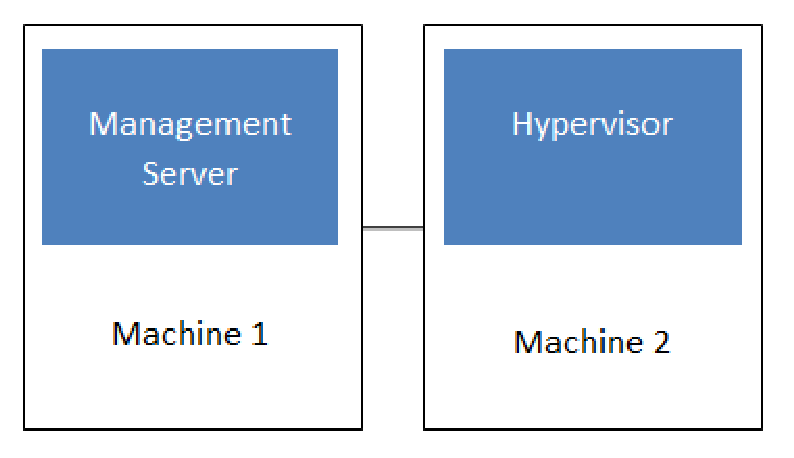
\includegraphics [keepaspectratio=true,scale=0.60]{figuras/cloudstack_minimal.eps}
\caption{Visão simplificada de uma instalação mínima do cloudstack}
\cite{cloudstack}.
\label{cloudstatck_minimal}
\end{figure}

Em modelo mais complexo, o cloudstack apresenta seu pontencial de disponibilidade escalabilidade e gerenciamento. Proporcionando uma modelagem de várias
infraestrutura em nuvens em uma determinada região. Desse modo o cloudstack possui os seguintes níveis de abstrações \cite{shape}:

\begin{itemize}
\item \textbf{Regiões:} são a primeira e maior unidade de escala de uma implementação de uma cloud com CloudStack. Uma Região consiste em multiplas Zonas de Disponibilidade, a segunda maior unidade de escala.
\item \textbf{Zonas: } Tipicamente existe apenas uma Zona por Data Center e cada Zona contem PODs, Hosts e Storage.
\item \textbf{Pods: } PODs tem propriedades lógicas e físicas com componentes como endereçamento IP e algoritmo de alocação de Máquinas Virutais sendo influenciados por PODs dentro de uma Zona.
\item \textbf{Clusters: } São simples grupos de servidores homogêneos combinados com um Storage Primário. Cada Cluster utiliza um mesmo tipo de hypervisor mas em uma Zona pode ceoxistir combinações de todos os hypervisores suportados. Cada Cluster utiliza um mesmo tipo de hypervisor mas em uma Zona pode ceoxistir combinações de todos os hypervisores suportados.
\item \textbf{Hosts: } Responsável por disponibilizar a camada de computação real em que Máquinas Virtuais são executadas.
\item \textbf{Storage Primário: }  onde os discos das Máquinas Virtuais residem e pode ser utilizado o disco local de um Host ou um storage compartilhado como NFS, iSCSI, Fiber Channel, etc.
\item \textbf{Storage Secundário:} onde é armazenado os Templates de Máquinas Virtuais, arquivos ISO e Snapshots e é utilizado o protocolo NFS para este Storage
\end{itemize}


\begin{figure}[!htb]
\centering
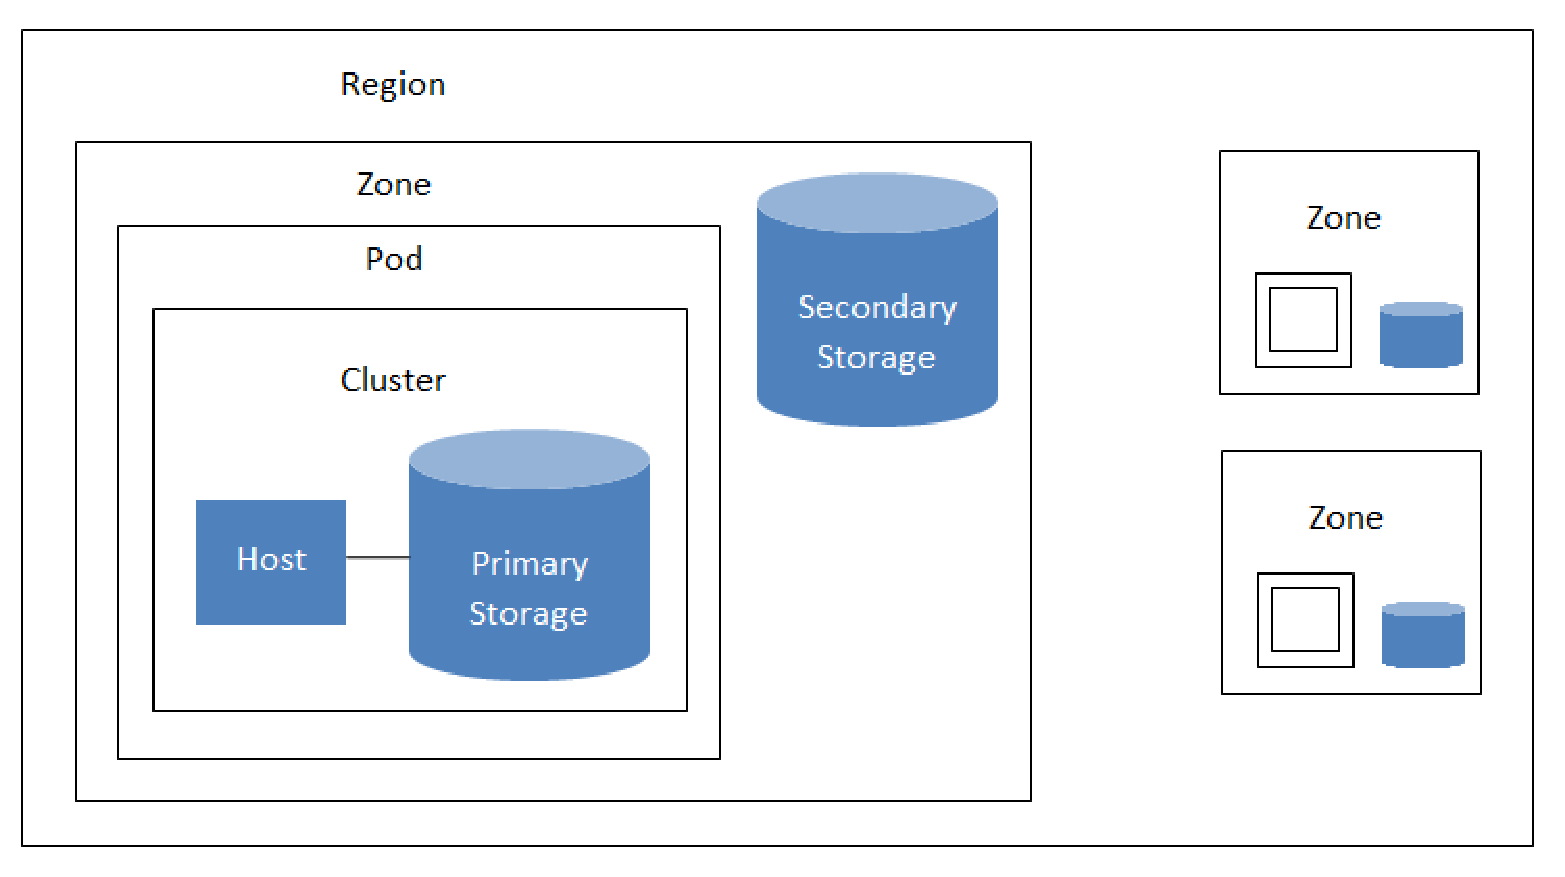
\includegraphics [keepaspectratio=true,scale=0.60]{figuras/cloudstack_structure.eps}
\caption{Visão geral da infraestrutura do Cloudstack}
\cite{cloudstack}.
\label{diagramacloudstack}
\end{figure}

Dessa maneira, afim de se ter um ambiente limpo e com um sistema operacional atualizado, efetuou-se a formtação do disco do servidor \textit{Solarian}, sendo em seguida instalado o sistema operacional \textit{Centos 7}. Assim, com o auxílio da documentação do cloudstack a instalação procedeu sem muitos problemas. Com instalação concluída, já era possível acessar a interface de gerenciamento dando continuidade com as configurações necessárias para criação de máquinas virtuais.Entretanto, a obrigatoriedade de configuração de todos os niveis de abstração apresentados logo a cima mostrou-se despendiosa e desnecessária para uma configuração mínima e também para a infraestrutura disponível no LAPPIS. Desse modo, alguns elementos separados que quando juntos não apresentaram o comportamento esperado. Um exemplo disso, era problemas recorrentes relacionados com a máquina virtual de sistema, reponsável pelas operações no storage secundário (referenciada por \textit{SSVM}), o que impossibilitava a criação de máquinas virtuais a partir de templates.Em resumo, mesmo com os problemas enfrentados, foi possível a criação de máquinas virtuais nessa plataforma, entretanto a configuração de vários elementos decorrente de sua abstração voltada para uma infraestrutura mais complexa, acabou por tornar difícil o gerenciamento e estabilização do ambiente como um todo, sendo considerado, para o caso em específico do LAPPIS, não sustentável.
   
%O cloudstack se mostrou de fácil instalação, usando no servidor físico um sistema operacional \textit{Centos 7}. Tão logo concluído, a interface de gerenciamento já se encontrava disponivel. O restante da configuração \textit{Ip's}, \textit{storage}, \textit{host}(servidor físico), deve ser feita via interface. E foi aí que encontrou-se dificuldade: A obrigatoriedade de configuração seus niveis de abstração mostrou-se bastante despendiosa para uma configuração mínima.Muitos elementos separados que quando se integram junto pode não se comportar da forma esperada.Outro fator que dificultou bastante na configuração foi suas \textit{VM's} criadas automaticamente.De maneira geral, foi possível a criação de máquinas virtuais, entretanto todo o ambiente demonstrou-se bastante instável, tendo assim bastante dificuldade na disponibilização de ambientes virtuais iniciais para testes.  

